
%%% Local Variables:
%%% mode: latex
%%% TeX-master: t
%%% End:

\chapter{绪论}
\label{cha1}

\section{引言}
近年来,随着经济和科技水平的快速提升,大量的海水养殖废水、工农业废水和人类生活污水排放使得海水富营养化现象不断加重,从而导致了有害赤潮的频繁发生,严重破坏了海洋生态系统的平衡,阻碍了海洋渔业的发展,并且极大威胁了人体健康和生命安全。

当前对藻类的研究工作主要依赖于显微观察技术,但传统的藻种识别以及分类技术主要由生物学者借助显微镜观察来完成。这一方式虽然具有较高的可靠性,但需要大量的操作者且对操作者专业知识水平要求较高,同时耗时费力,效率较低,在样本数较多的情况下难以快速分析。随着图像处理技术和计算机水平的发展,结合生物形态特征的显微图像处理技术,由于其识别准确率高、处理操作过程简单快捷的特点,受到了国内外的广泛关注。

在借助于传统方法的藻类图像识别和分类过程中,首要工作是对原始藻类显微图像进行图像分割,分离出图像中的藻类细胞区域,因此对藻类显微图像进行分割对于后续分类工作有着非常重要的意义。
本文的研究对象是角毛藻属藻,角毛藻属在海洋浮游硅藻属中占据着重要的地位,有约400个物种,其数量庞大、种类繁多并且遍布世界各个海域中,其生物形态特征主要集中在细而长的角毛上。探索角毛藻显微图像的分割方法对角毛藻属间不同物种分类具有重要影响。

\section{国内外研究现状}
目前,国内外许多研究者们对藻类显微的图像分割进行了不少相关研究,并取得了显著成果。例如,Jalba\cite{jalba2003automatic}\cite{jalba2004automatic}等提出了一种利用基于数学形态学工具的标记分水岭算法,它可以成功用于实现自动硅藻显微图像的分割;Rodenacker\cite{rodenacker2006automatic}等人通过使用基于阈值的方法从显微图像中分割出水溶样本;Blaschko\cite{blaschko2005automatic}等对流式细胞摄像技术产生的原位图像使用多种特征和多重分类器结合的方法来实现分割;Sosik和Olson\cite{sosik2007automated}等针对流式细胞成像技术产生的相位一致图像采用了简单的基于阈值的边缘检测来提取浮游植物细胞的特征;Luo\cite{luo2011automatic}等使用了Canny边缘检测结合稳健回归的方法来分割显微图像中的圆形硅藻;Verikas\cite{verikas2012phase}等采用了模糊C均值聚类算法对浮游植物显微图像中的代替最小原甲藻的圆形目标进行分割;Soh\cite{soh2008segmentation}等则提出了使用均值漂移聚类和基于图的聚类合并的浮游生物图像分割方法;Su\cite{cuiping2010system}等选择了改进区域生长算法分割用于利用边缘信息来识别海洋浮游植物显微图像;Kloster\cite{kloster2014sherpa}等介绍了用于硅藻和其他目标的图像分割和轮廓特征提取工具SHERPA,这种工具使用了五个不用的步骤,包括Otsus阈值、Canny 边缘检测,自动阈值选择(RATS)和自适应阈值;Gelzinis\cite{gelzinis2015novel}等提出了一种基于活动轮廓模型(ACM)用于准确提取细胞轮廓来进行浮游植物的分割。
\section{课题背景与研究意义}
角毛藻属是海洋浮游植物的重要组成部分,具有种类繁多、数量庞杂、单位体积小、大量聚集且形状复杂的特点,是许多海洋动物的饵料,但其中有的角毛藻(如扁面角毛藻和旋链角毛藻等)则是引发有害赤潮的主要因素。因此,角毛藻属的种类构成对海洋环境以及海洋生态系统中的其它生物有着十分重要的影响,具有很大的研究价值。

实现角毛藻显微图像的分割有助于对角毛藻属进行物种分类,从而控制并避免赤潮的发生。然而,由于角毛藻属细胞在显微镜下复杂多样并且呈现出明暗相间、边界模糊的现象,传统的图像分割算法对角毛藻显微图像分割难以取得令人满意的效果。所以,实现该课题对保持维护生态环境及进行角毛藻属分类的学术研究有着一定的意义。


 \section{主要工作内容及安排}
 本文以角毛藻为研究对象,针对角毛藻属独特的生物形态学特征和显微图像的特点,利用灰度平面方向角模型和支持向量机相结合的方式对角毛藻显微图像开展一系列分割工作,本文具体分割方法流程图如图\ref{flowchart}所示:

   \begin{figure}[ht!]
   \centering
  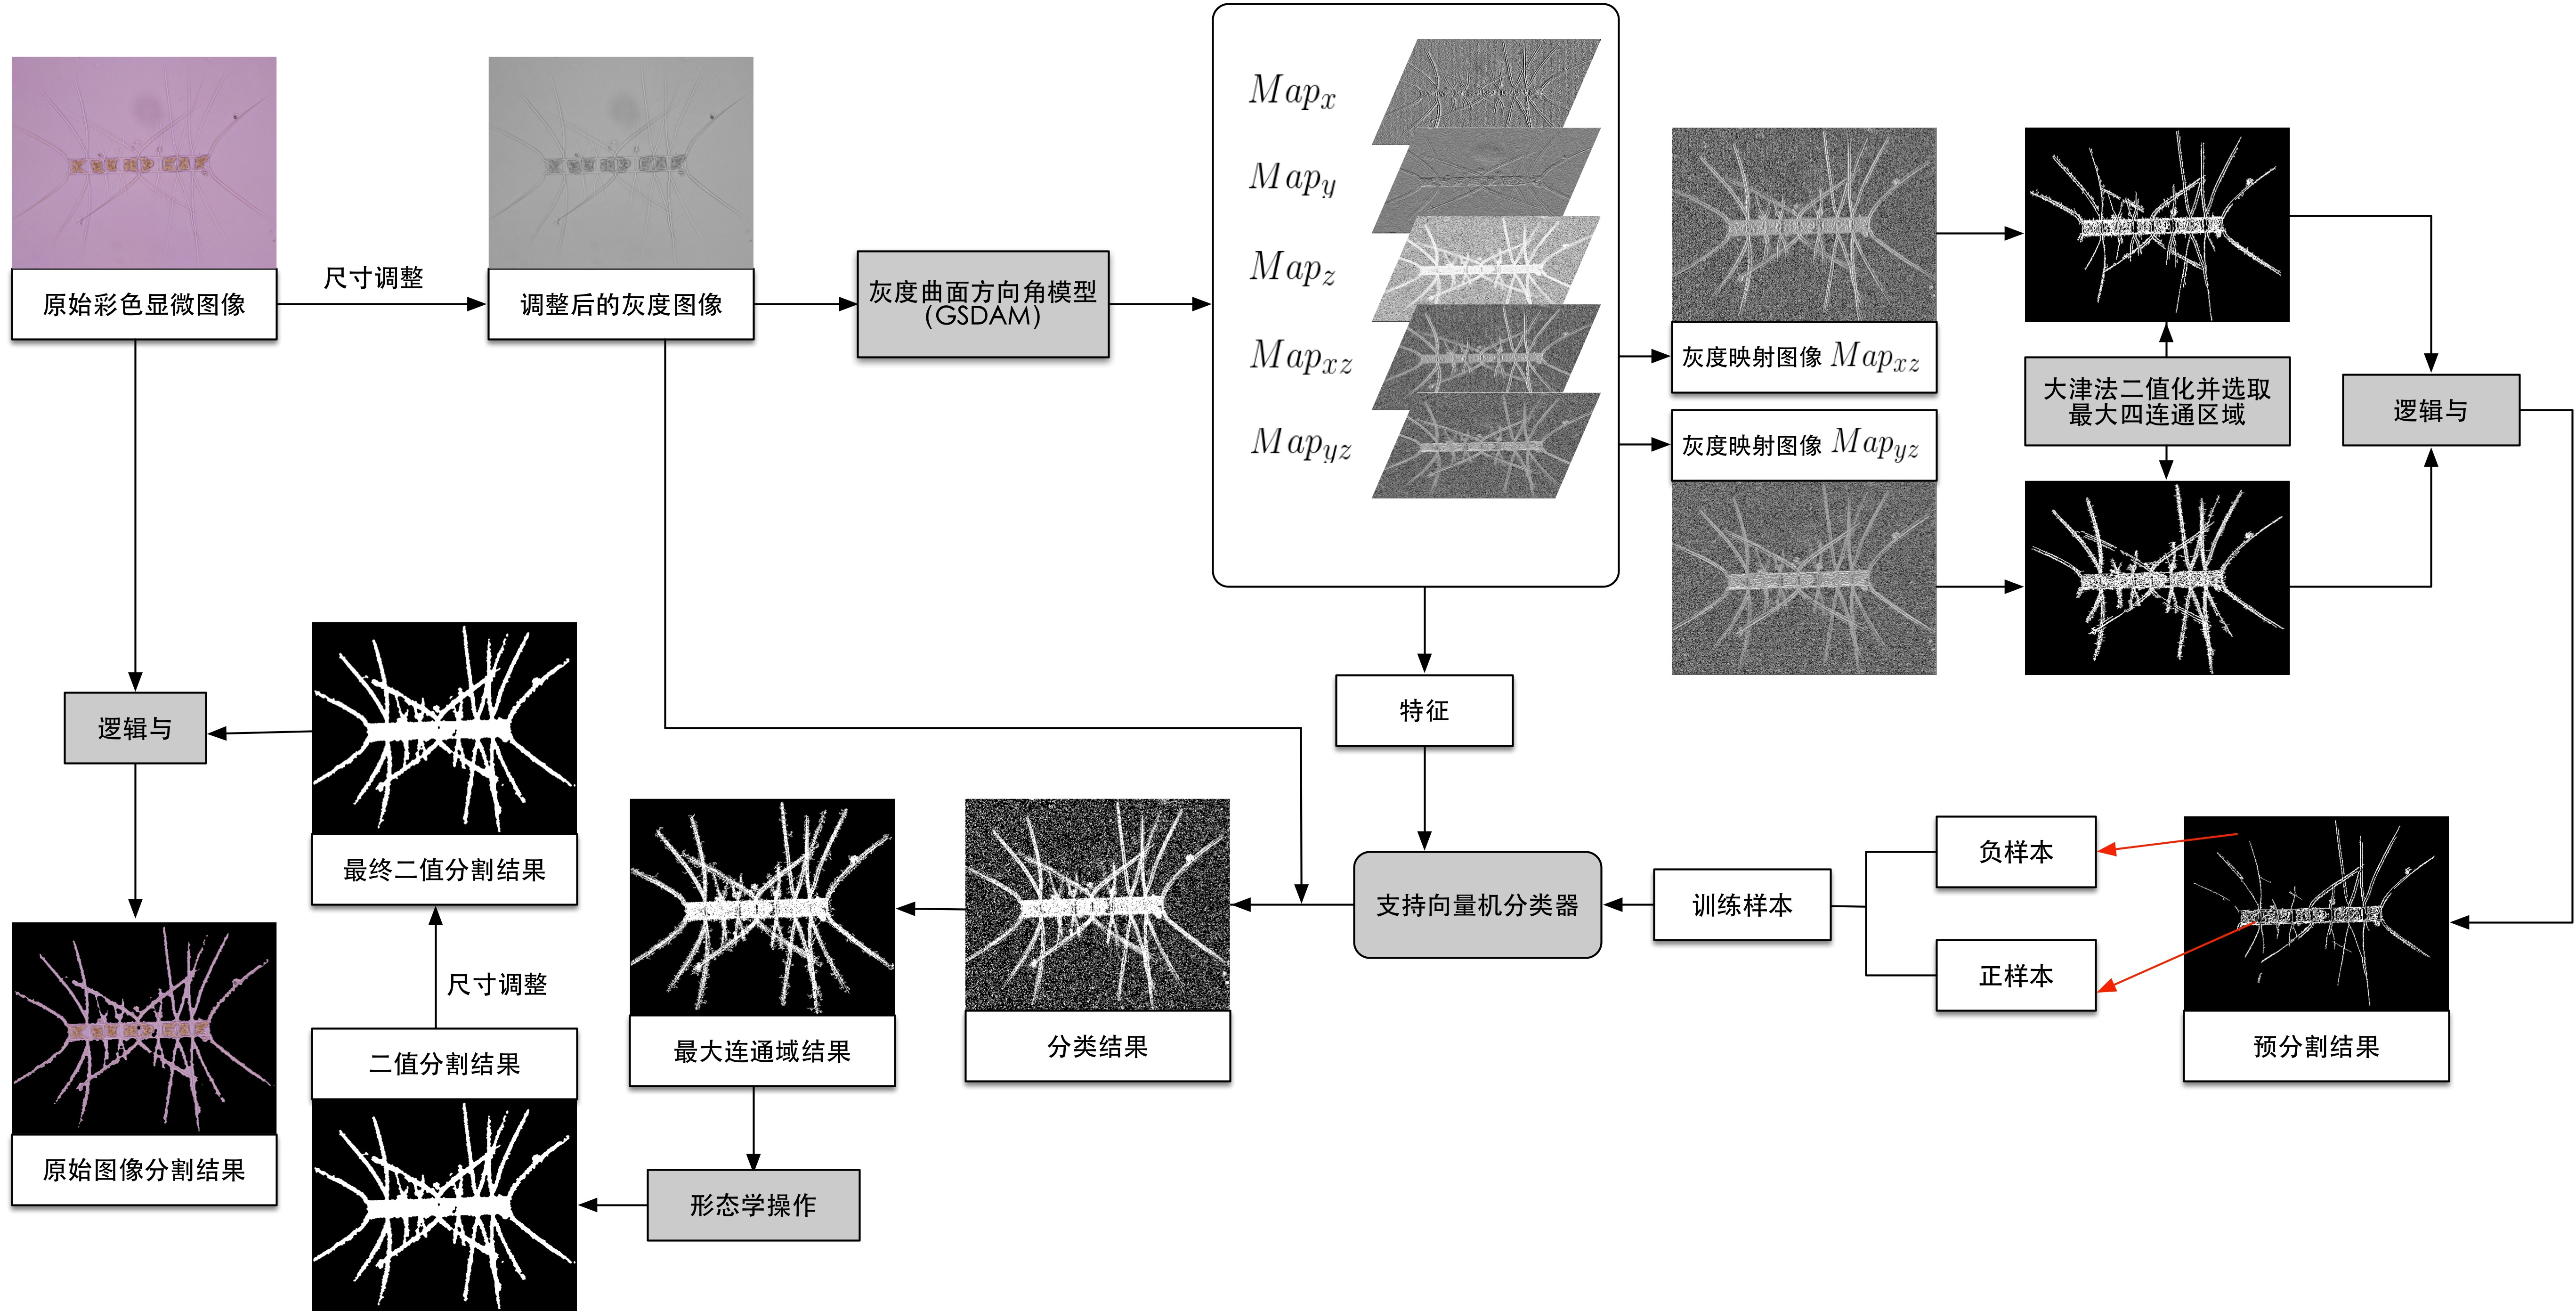
\includegraphics[width=0.9\linewidth]{flowchart.jpg}
  \caption{基于灰度曲面方向角模型和支持向量机的角毛藻显微图像分割算法流程图}
    \label{flowchart}
 \end{figure}

本文的内容安排如下:

第一章为绪论,主要介绍了藻类图像分割的国内外研究现状、课题背景与研究意义和本文的主要工作安排。

第二章为角毛藻显微图像的特征提取,主要根据角毛藻独特的生物形态学特征使用灰度曲面方向角模型(Grayscale Surface Direction Angle Model)来提取角毛藻的特征,使用该模型提取的特征含有大量的角毛藻角毛信息。

第三章为连通区域的预分割,主要运用大津法(Otsu)并选取最大连通域对图像进行预分割来生成后续支持向量机训练过程需要的训练样本。

第四章为支持向量机(Support Vector Machines)分类与后续处理,本文通过将分割问题转化为像素分类问题的形式,主要使用支持向量机来对角毛藻显微图像中的每个像素进行分类,最终完成目标(角毛藻)和背景(图像中除了角毛藻之外的其余部分)的二分类问题,最后通过一些简单的后续处理操作得到最终的分割结果。

第五章是总结和展望,分析总结了本文的工作并对今后的研究工作进行展望。

